\documentclass[lettersize,journal]{IEEEtran}

\usepackage{amsmath,amssymb,amsfonts,mathtools}
\usepackage{graphicx}
\usepackage{booktabs}
\usepackage{multirow}
\usepackage{array}
\usepackage{cite}
\usepackage{url}
\usepackage{xcolor}
\usepackage{tikz}
\usetikzlibrary{arrows.meta,positioning,fit,shapes.geometric}
\usepackage{algorithm}
\usepackage[noend]{algpseudocode}
\usepackage[hidelinks]{hyperref}

\newcommand{\R}{\mathbb{R}}
\newcommand{\E}{\mathbb{E}}
\newcommand{\vect}[1]{\boldsymbol{#1}}
\newcommand{\norm}[1]{\left\lVert #1\right\rVert}
\newcommand{\todo}[1]{\textcolor{red}{[TODO: #1]}}

\begin{document}

\title{Meta-Guided Action-Manifold Smoothing for Secure Ackermann Vehicle Platoons under Hybrid Attacks}

\author{Zhiwei Xia, Chun Liu, Xiaoqiang Ren, Xiaofan Wang, and Youmin Zhang%
\thanks{This manuscript is a current project draft prepared from the AMS implementation and verified simulation records. The independent multi-training-seed revalidation is still in progress and is not treated as completed evidence in this draft.}}

\maketitle

\begin{abstract}
Connected vehicle platoons must preserve both geometric path tracking and inter-vehicle coordination when communication and actuation channels are attacked. Hybrid denial-of-service and false-data-injection attacks are especially damaging because they can distort local observations, executed commands, and the reward used by a learning controller. Existing meta-gradient reward shaping corrects the direction of policy learning by comparing attacked observations with privileged physical performance, but it does not explicitly regularize the local geometry of action updates. This paper introduces Meta-Guided Action-Manifold Smoothing (Meta-AMS), a hierarchical security-learning framework for a five-vehicle Ackermann platoon. A physics-aware reward teacher provides the task-level direction, while an auxiliary twin action-value model evaluates a feasible neighborhood of joint speed--steering actions. Orthogonal neighborhood directions, Ackermann feasibility projection, executed-command anchoring, and a warm-up/ramp schedule are combined with HAPPO updates. We formulate a conditional local ultimate-boundedness argument for the normalized platoon tracking error and give a complete training and evaluation protocol with progressive hybrid attacks. In the available verified single-training-chain result, Meta-AMS completes the clean task and all attack levels through hard-a with zero collision and road-termination rates, and achieves 0.75 whole-platoon completion at hard-b. The current orthogonal pilot indicates a benefit from combining the meta teacher with AMS, while the standalone AMS cell remains a diagnostic failure case and is therefore not used to claim a final causal effect.
\end{abstract}

\begin{IEEEkeywords}
Vehicle platooning, Ackermann steering, hybrid cyber attacks, multi-agent reinforcement learning, reward shaping, action-manifold smoothing, HAPPO, safety-critical control.
\end{IEEEkeywords}

\section{Introduction}
\IEEEPARstart{V}{ehicle} platooning couples multiple autonomous vehicles through communication, motion constraints, and a shared spatial task. A controller must maintain safe gaps while every vehicle follows the same path and completes the maneuver. This requirement becomes substantially harder when the platoon uses learned policies and the communication channels are exposed to denial-of-service (DoS) and false-data-injection (FDI) attacks. DoS can hold or remove information, whereas FDI can make a plausible but physically incorrect relative state or command appear valid. Under a hybrid attack, a reward computed from corrupted observations may also become misaligned with the true physical objective.

The reference MGRS study \cite{xia2026security} addresses this misalignment with a hierarchical meta-gradient reward teacher. Its upper layer observes trusted physical quantities during centralized training and adapts a reward-shaping function; its lower layer learns decentralized policies from attacked observations. This principle is powerful at the task level, but a second failure mode remains: even when the reward direction is corrected, a policy update may move too far in the local speed--steering action geometry. The problem is particularly visible for an Ackermann platform. A perturbation in a normalized steering coordinate changes curvature, front-wheel geometry, and the spacing evolution of following vehicles. Treating each action coordinate as an unconstrained Euclidean direction can therefore create a locally high-value action estimate that is physically inconsistent with the vehicle.

This paper develops Meta-Guided Action-Manifold Smoothing (Meta-AMS). The method retains the trusted outer reward direction from meta-gradient shaping and adapts Action Manifold Smoothing (AMS) \cite{lin2026actionmanifold} to an on-policy multi-agent HAPPO update. The action-manifold critic evaluates symmetric, feasible neighborhoods around the executed joint action. The security motivation follows the broader resilience literature on connected vehicles \cite{ju2022survey,zhao2024safeguard}. The proposed mechanism has four design principles:

\begin{enumerate}
\item The meta teacher corrects the \emph{direction} of learning using clean physical performance, rather than asking the attacked reward to describe its own corruption.
\item AMS corrects the \emph{local geometry} of the policy update by smoothing an action-value estimate over feasible speed--steering neighborhoods.
\item The Ackermann map is part of the learning constraint: rear wheels receive drive velocity targets only, and front knuckles receive the coupled left/right steering targets.
\item Clean imitation and retention are used before attack escalation; every attack stage is unlocked only when the complete five-vehicle maneuver satisfies completion, safety, and dwell gates.
\end{enumerate}

The contributions of this draft are:

\begin{itemize}
\item a unified Meta-AMS formulation for secure spatial path following with a five-vehicle Ackermann platoon under hybrid DoS--FDI attacks;
\item a geometry-aware AMS update with twin critics, orthogonal neighborhood sampling, feasible projection, executed-command anchoring, and advantage warm-up;
\item a conditional local ultimate-boundedness analysis that separates the trusted task-level teacher signal from the local action-smoothing residual;
\item a reproducible simulation protocol and a disk-traceable comparison. The completed Meta-AMS ladder reaches 0.75 whole-platoon completion at hard-b, while collision, road-boundary violation, and road termination remain zero in the reported matrix;
\item an honest pilot interpretation of the current orthogonal ablation. The independent training-seed revalidation is in progress and is deliberately excluded from the claims made here.
\end{itemize}

\section{Problem Formulation}
\subsection{Five-Vehicle Ackermann Platoon}
Consider one leader and four followers, indexed by $i\in\{1,\ldots,5\}$ for the five physical vehicles. The local planar state is
\begin{equation}
\vect{x}_i=[x_i,y_i,\psi_i,v_i]^{\mathsf T},
\end{equation}
where $(x_i,y_i)$ is the body reference position, $\psi_i$ is yaw, and $v_i$ is the forward speed. With wheelbase $L$ and front steering angle $\delta_i$, the kinematic core follows the standard Ackermann bicycle abstraction \cite{rajamani2012vehicle}:
\begin{equation}
\dot{x}_i=v_i\cos\psi_i,\quad
\dot{y}_i=v_i\sin\psi_i,\quad
\dot{\psi}_i=\frac{v_i}{L}\tan\delta_i,\quad
\dot{v}_i=a_i+w_i.
\label{eq:ackermann}
\end{equation}
The rear steering angle is identically zero. The policy action is a normalized pair
\begin{equation}
\vect{a}_i=[a_i^{v},a_i^{\delta}]^{\mathsf T}\in[-1,1]^2,
\end{equation}
which is mapped to center speed and center steering by
$v_i=v_{\max}a_i^v$ and $\delta_i=\delta_{\max}a_i^\delta$. The implementation uses $L=0.14325$ m, $v_{\max}=1.20$ m/s, and $\delta_{\max}=0.32$ rad.

For track width $T$, the two front steering targets are generated from the center steering command:
\begin{align}
\delta_{i,L}
&=\tan^{-1}\left(\frac{L\tan\delta_i}
 {L-\frac{T}{2}\tan\delta_i}\right),\\
\delta_{i,R}
&=\tan^{-1}\left(\frac{L\tan\delta_i}
 {L+\frac{T}{2}\tan\delta_i}\right).
\label{eq:inner_wheel}
\end{align}
The rear axle receives only wheel angular-velocity targets. Thus, the action interface itself enforces the front-steering-only Ackermann structure.

\subsection{Shared Spatial Lane-Change Path}
All five vehicles follow one geometric reference. The reference is a quintic spatial transition. For a vehicle-local longitudinal coordinate $x$, define
\begin{equation}
\zeta(x)=\operatorname{clip}\left(\frac{x-x_s}{\ell},0,1\right),\qquad
h(\zeta)=10\zeta^3-15\zeta^4+6\zeta^5,
\end{equation}
and
\begin{equation}
y_{\rm ref}(x)=y_s+(y_e-y_s)h(\zeta(x)).
\label{eq:quintic}
\end{equation}
The verified protocol uses $x_s=-7.75$ m, $\ell=6.0$ m, $y_s=-0.065$ m, and $y_e=-1.160$ m. The five initial longitudinal positions are separated by 1.50 m. The reference provides a common centerline and heading target, while each follower additionally receives predecessor-relative features.

The local observation contains predecessor-relative position and velocity, ego velocity and yaw rate, centerline and heading error, relative heading, and a vehicle-role identifier. The centralized critic receives the joint observation, while each actor uses only its local attacked observation. This is a centralized-training/decentralized-execution (CTDE) design \cite{lowe2017multi,yu2022surprising,he2022happo}.

\subsection{Hybrid DoS--FDI Attack}
Let $\vect{o}_i$ denote the clean local observation and $\vect{u}_i$ the raw command. A general hybrid attack interface can represent FDI vectors and DoS probabilities as
\begin{equation}
\vect{\xi}_i=G_{\theta_G}(\vect{z}_i,\vect{o}_i)
=[\vect{f}_{p,i},q_{p,i},\vect{f}_{a,i},q_{a,i}].
\end{equation}
The attacked observation and command are
\begin{align}
\widetilde{\vect{o}}_i
&=\boldsymbol{\beta}_{p,i}\odot\vect{o}_i+\vect{f}_{p,i}
  +(\mathbf{1}-\boldsymbol{\beta}_{p,i})\odot\vect{o}_{i,\rm hold},\\
\widetilde{\vect{u}}_i
&=\beta_{a,i}\vect{u}_i+\vect{f}_{a,i}
  +(1-\beta_{a,i})\vect{u}_{i,\rm hold},
\label{eq:attack}
\end{align}
where the binary masks are sampled from the selected attack process. The reported matrices use the bounded \texttt{profile} attack mode: stage-specific FDI and DoS budgets are sampled from the fixed evaluation protocol, while the CAGAN/generator mode is an available but unreported extension. Thus the results should be described as hybrid profile DoS--FDI experiments, not as evidence from an actively trained conditional attack generator. The evaluation ladder increases the observation FDI, command FDI, and DoS budgets from \textit{off} through \textit{light}, \textit{easy}, \textit{medium}, and \textit{hard}. At hard-b, the protocol uses position FDI 4.0, acceleration FDI 1.3, and DoS rate 0.18.

\subsection{Strict Whole-Platoon Completion}
The maneuver is considered complete only when every vehicle reaches at least 99\% spatial progress, with centerline error at most 0.12 m, heading error at most 0.12 rad, predecessor gap error at most 0.35 m, pair lateral error at most 0.20 m, pair distance at least 0.30 m, and no road-boundary exceedance. The conditions must persist for a 2.0 s dwell. This whole-platoon criterion is stricter than a mean spacing score and is motivated by string-stability concerns in platoons \cite{swaroop1996string}. We report the whole-platoon completion rate, not the average number of vehicles that happen to reach the target.

\section{Meta-Guided Action-Manifold Smoothing}
\subsection{Bi-Level Task Direction}
Let $\theta$ denote the decentralized policy parameters and $\phi$ the reward-teacher parameters. The attacked local reward is augmented by a learned shaping term:
\begin{equation}
R_{\phi}(\widetilde{\vect{o}}_i,\vect{u}_i)
=R_{\rm env}(\widetilde{\vect{o}}_i,\vect{u}_i)
 +F_{\phi}(\widetilde{\vect{o}}_i,\vect{u}_i).
\label{eq:shaped_reward}
\end{equation}
During centralized training, a trusted physical score is computed from true states and executed commands:
\begin{equation}
\mathcal{L}_{\rm phy}
=\frac{1}{5}\sum_{i=1}^{5}
\left(
\lambda_p e_{p,i}^2+
\lambda_v e_{v,i}^2+
\lambda_a e_{a,i}^2+
\lambda_c e_{c,i}^2+
\lambda_\psi e_{\psi,i}^2+
\lambda_j \dot{a}_i^2+
\lambda_u\norm{\vect{u}_i}^2
\right)
 +\lambda_{\rm col}I_{\rm col}.
\label{eq:physical_loss}
\end{equation}
The ideal lower-level and upper-level problems are
\begin{align}
\theta^*(\phi)&\in\arg\max_{\theta}J_{\rm in}(\theta;\phi),\\
\min_{\phi}\quad &J_{\rm out}(\phi)=J_{\rm phy}(\theta^*(\phi)).
\label{eq:bilevel}
\end{align}
This preserves the central idea of meta-gradient reward shaping \cite{xia2026security,finn2017model} and the safety-oriented view that performance constraints should be represented explicitly \cite{tessler2019reward}: the teacher is updated from trusted post-update physics, while deployment uses only the learned students.

For a one-step differentiable surrogate,
\begin{equation}
\bar{\theta}^{+}
=\theta^{-}+\alpha g_{\rm in}(\theta^{-},\phi),
\end{equation}
the first-order outer direction is
\begin{equation}
\nabla_{\phi}J_{\rm out}
=\left(\frac{\partial\bar{\theta}^{+}}{\partial\phi}\right)^{\mathsf T}
\nabla_{\bar{\theta}^{+}}J_{\rm phy}.
\label{eq:meta_gradient}
\end{equation}
The implementation uses a stable proxy based on normalized physical-score changes and the covariance between centered physical advantages and centered teacher outputs. A warm-up and ramp prevent the teacher from dominating before the retention-initialized policy has learned the basic maneuver.

\subsection{Action-Manifold Critic}
The AMS module receives a centralized observation $\vect{s}$ and a joint action $\vect{a}\in\R^{10}$ formed by five speed--steering pairs. It learns two auxiliary action-value functions $Q_1$ and $Q_2$. Let $\{\vect{d}_j\}_{j=1}^{K}$ be orthonormal directions obtained from a QR factorization and let $\epsilon=r\ell_a$, where $r$ is the neighborhood radius and $\ell_a$ is the normalized action limit. The feasible neighbors are
\begin{equation}
\vect{a}_{j}^{\pm}
=\Pi_{\mathcal{A}_{\rm Ack}}
\left(\vect{a}\pm\epsilon\vect{d}_j\right),
\qquad j=1,\ldots,K.
\label{eq:neighbors}
\end{equation}
The projection $\Pi_{\mathcal{A}_{\rm Ack}}$ clips normalized speed and steering, limits curvature, and preserves the speed--steering pair structure. The smoothed target value is
\begin{equation}
\overline{Q}^{\,t}(\vect{s},\vect{a})
=\frac{1}{2K}\sum_{j=1}^{K}
\min_{q\in\{1,2\}}
\left[
Q_q^{t}(\vect{s},\vect{a}_{j}^{+})
+Q_q^{t}(\vect{s},\vect{a}_{j}^{-})
\right],
\label{eq:smooth_q}
\end{equation}
and the clipped temporal-difference target is
\begin{equation}
y=r+\gamma m\,\overline{Q}^{\,t}(\vect{s}',\vect{a}'),
\label{eq:ams_target}
\end{equation}
where $m$ is the continuation mask. Each critic is trained with a Huber loss against $y$, followed by a Polyak target update.

The action anchor is the physically executed action, rather than a relabeled projection of the stored transition. The local AMS advantage for the actor update is
\begin{equation}
A_{\rm AMS}
=\min(Q_1,Q_2)(\vect{s},\vect{a}_{\rm exec})
-\overline{Q}(\vect{s},\Pi_{\mathcal{A}_{\rm Ack}}(\vect{a}_{\pi}))
-\rho\sqrt{\operatorname{Var}(Q_{\rm neigh})},
\label{eq:ams_advantage}
\end{equation}
where $\rho\geq 0$ is an optional local-risk coefficient. The current verified configuration uses $K=8$, radius $r=0.25$, Huber parameter 0.3, target smoothing $\tau=0.01$, and $\rho=0$.

\subsection{HAPPO Update and Warm-Up}
Let $A_{\rm HAPPO}$ be the normalized sequential-policy advantage. The actor receives
\begin{equation}
A_{\rm total}
=\operatorname{Norm}\left(
A_{\rm HAPPO}
+\lambda_k\operatorname{Norm}(A_{\rm AMS})
\right),
\label{eq:total_advantage}
\end{equation}
where
\begin{equation}
\lambda_k=
\begin{cases}
0,& k\leq k_{\rm warm},\\
\lambda_{\max}\min\left(\dfrac{k-k_{\rm warm}}{k_{\rm ramp}},1\right),& k>k_{\rm warm}.
\end{cases}
\label{eq:ramp}
\end{equation}
The runner defaults are $\lambda_{\max}=0.10$, 50 warm-up updates, and a 100-update ramp, but the verified matrix launcher overrides these values to $\lambda_{\max}=0.02$, 5 warm-up updates, and a 15-update ramp for the reported short stage budgets. Meta-AMS therefore adds a bounded local action signal to a trust-region-style policy update \cite{schulman2017proximal,yu2022surprising}, rather than replacing the task reward or the HAPPO objective.

\subsection{Training Algorithm}
Algorithm~\ref{alg:metaams} summarizes the complete sequence. The attack curriculum and the expert-retention warm start are part of the algorithm, because abruptly enabling the hard attack before the five vehicles can perform the clean spatial maneuver confounds security learning with basic path acquisition.

\begin{algorithm}[t]
\caption{Meta-AMS training under progressive hybrid attacks}
\label{alg:metaams}
\begin{algorithmic}[1]
\Require BC/retention initialization $\theta$, teacher $\phi$, AMS critics $Q_1,Q_2$, attack profile (or optional generator $G$)
\For{attack stages $\ell\in\{\mathrm{off},\mathrm{light},\ldots,\mathrm{hard\mbox{-}b}\}$}
  \State Set the stage attack budgets and reset the strict completion gate
  \For{student update $k=1,\ldots,K_\ell$}
    \State Roll out five Ackermann vehicles with attacked local observations
    \State Store raw actions and physically executed actions
    \State Compute attacked rewards and trusted physical teacher scores
    \State Update the HAPPO students with the retention-aware shaped reward
    \State Sample feasible AMS neighbors and update twin action-value critics
    \State Add the warm-started AMS advantage using \eqref{eq:total_advantage}
    \If{teacher boundary is active}
      \State Update $\phi$ using the normalized physical-score/teacher-output proxy
    \EndIf
    \State If generator mode is enabled, update $G$ and its discriminator; otherwise retain the fixed profile sampler
  \EndFor
  \State Evaluate clean and attacked environments with fixed evaluation seeds
  \If{all completion, dwell, collision, and road gates pass}
    \State Promote the checkpoint to the next attack stage
  \Else
    \State Keep the last passing checkpoint and record the failure diagnostics
  \EndIf
\EndFor
\end{algorithmic}
\end{algorithm}

\section{Conditional Stability Interpretation}
The proposed learning rule is not an unconditional global safety certificate. Its control interpretation is conditional and local, consistent with the meta-gradient framework in \cite{xia2026security} and local safety-filter reasoning \cite{ames2019control,ghiasi2020resilient}. Let $e_p,e_v,e_\psi,e_c$ collect platoon spacing, velocity, heading, and centerline errors, and define the scaled vector
\begin{equation}
\bar{\vect e}=
\operatorname{diag}(s_p I,s_v I,s_\psi I,s_c I)^{-1}
\operatorname{col}(e_p,e_v,e_\psi,e_c).
\end{equation}
Let $\bar{\vect\omega}$ collect bounded FDI, external disturbance, held-packet error, and finite policy residual. We use the following local assumptions.

\textbf{Assumption 1 (bounded admissible attack).} The FDI and DoS budgets are finite, and the induced hold error remains bounded over the considered local operating domain.

\textbf{Assumption 2 (local dissipativity).} For the trained closed loop, there is a positive definite function $V(\bar{\vect e})$ and constants $c_1,c_2,\alpha,c_\omega,c_{\rm cl}>0$ such that
\begin{equation}
c_1\norm{\bar{\vect e}_k}^2
\leq V(\bar{\vect e}_k)
\leq c_2\norm{\bar{\vect e}_k}^2,
\end{equation}
and
\begin{equation}
V(\bar{\vect e}_{k+1})-V(\bar{\vect e}_k)
\leq-\alpha V(\bar{\vect e}_k)
+c_\omega\norm{\bar{\vect\omega}_k}^2
+c_{\rm cl}\varepsilon_{\rm cl}^2.
\label{eq:lyap}
\end{equation}

\textbf{Proposition 1 (conditional local ultimate boundedness).} Under Assumptions 1--2 and $\norm{\bar{\vect\omega}_k}\leq\bar{\omega}$, every trajectory that remains in the local operating domain satisfies
\begin{equation}
V(\bar{\vect e}_k)
\leq(1-\alpha)^kV(\bar{\vect e}_0)
+\frac{1-(1-\alpha)^k}{\alpha}
\left(c_\omega\bar{\omega}^2+c_{\rm cl}\varepsilon_{\rm cl}^2\right),
\end{equation}
and hence
\begin{equation}
\limsup_{k\rightarrow\infty}\norm{\bar{\vect e}_k}
\leq
\sqrt{\frac{c_\omega\bar{\omega}^2+c_{\rm cl}\varepsilon_{\rm cl}^2}{\alpha c_1}}.
\label{eq:uub}
\end{equation}
Consequently, the prescribed componentwise margins are achieved whenever the right-hand side of \eqref{eq:uub}, multiplied by the corresponding scale, is below the spacing, velocity, heading, and centerline tolerances.

\emph{Discussion.} AMS contributes to this interpretation in two ways. First, $\Pi_{\mathcal{A}_{\rm Ack}}$ limits the counterfactual action set used by the auxiliary critic, so the smoothing residual is evaluated over feasible curvature and speed changes. Second, the neighborhood variance term in \eqref{eq:ams_advantage} can be used as a local uncertainty penalty when $\rho>0$. The proposition still depends on the local closed-loop dissipativity condition; the simulation gates are empirical tests of that condition rather than a replacement for it.

\section{Simulation Protocol}
\subsection{Environment and Warm Start}
Experiments use NVIDIA Isaac Sim/Isaac Lab with a physics-based planar environment \cite{isaacsim2022}. The platoon contains five Wheeltec mini Ackermann vehicles. The action implementation resolves exactly two rear wheel joints and two front steering joints for every vehicle; rear joints receive velocity targets and front knuckles receive the coupled steering targets in \eqref{eq:inner_wheel}. A real trajectory is used for behavior-cloning warm start. The recorded BC checkpoint contains 10,995 samples, with validation speed MAE $7.23\times10^{-4}$ and steering MAE $6.69\times10^{-3}$ in normalized units.

The training protocol initializes each cell from the same simulator-executed trajectory BC checkpoint and applies fixed behavior-cloning and reference-policy KL retention penalties. The code supports a progressive retention/expert-exit schedule, but both schedule switches are disabled in the verified orthogonal matrix; expert blend ratios are also zero during the reported attack stages. Therefore the present matrix demonstrates BC/retention warm-started attack adaptation, not a completed causal evaluation of progressive expert withdrawal. A dedicated schedule ablation is required before making the stronger gradual-exit claim. The clean gate requires all five vehicles to complete the same spatial lane change and hold the terminal condition for 2 s. The same BC initialization, physical path, 32 training environments, 16 evaluation environments, and 40-update stage budget are used in the verified orthogonal comparison. Each attack level is evaluated with three fixed environment/attack seed pairs: $(42,3407)$, $(3407,9917)$, and $(777,17011)$.

\subsection{Attack Ladder and Metrics}
The nine evaluated levels are \textit{off}, \textit{light}, \textit{easy-0}, \textit{easy-a}, \textit{easy-b}, \textit{med-a}, \textit{med-b}, \textit{hard-a}, and \textit{hard-b}. A checkpoint is promoted only if the clean gate and the current attacked gate pass. We report:
\begin{enumerate}
\item whole-platoon completion rate over the evaluation environments;
\item the minimum completion rate among the three evaluation seeds;
\item episode return;
\item collision rate, road-boundary violation rate, and road-termination rate;
\item qualitative evidence from the common spatial trajectory, top-down path, and physical front-steering traces.
\end{enumerate}

\begin{figure*}[t]
\centering
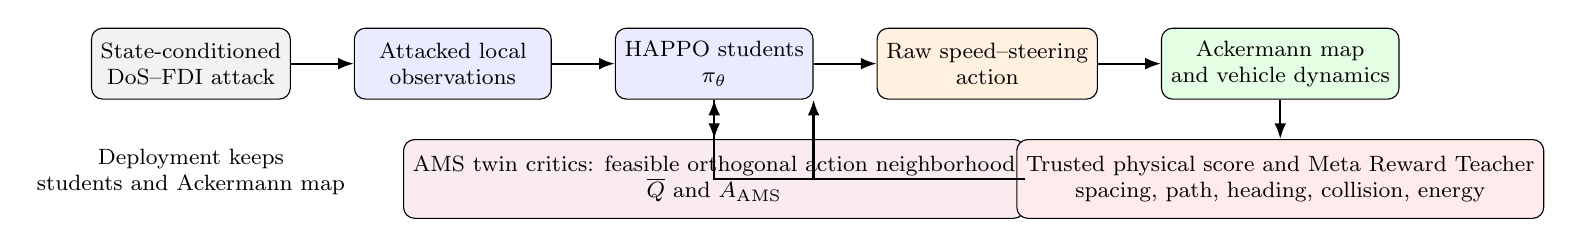
\begin{tikzpicture}[
  node distance=5mm and 8mm,
  box/.style={draw, rounded corners, align=center, minimum height=9mm, minimum width=25mm, font=\footnotesize},
  wide/.style={draw, rounded corners, align=center, minimum height=10mm, minimum width=38mm, font=\footnotesize},
  arrow/.style={-{Latex[length=2mm]}, thick}
]
\node[box, fill=gray!10] (attack) {State-conditioned\\DoS--FDI attack};
\node[box, right=of attack, fill=blue!8] (obs) {Attacked local\\observations};
\node[box, right=of obs, fill=blue!8] (student) {HAPPO students\\$\pi_\theta$};
\node[box, right=of student, fill=orange!12] (raw) {Raw speed--steering\\action};
\node[box, right=of raw, fill=green!10] (vehicle) {Ackermann map\\and vehicle dynamics};
\node[wide, below=of student, fill=purple!8] (ams) {AMS twin critics: feasible orthogonal action neighborhood\\$\overline Q$ and $A_{\rm AMS}$};
\node[wide, below=of vehicle, fill=red!8] (teacher) {Trusted physical score and Meta Reward Teacher\\spacing, path, heading, collision, energy};
\draw[arrow] (attack) -- (obs);
\draw[arrow] (obs) -- (student);
\draw[arrow] (student) -- (raw);
\draw[arrow] (raw) -- (vehicle);
\draw[arrow] (vehicle) -- (teacher);
\draw[arrow] (teacher.west) -| (student.south);
\draw[arrow] (student.south) -- (ams.north);
\draw[arrow] (ams.east) -| (student.south east);
\node[below=of attack, align=center, font=\footnotesize] (deploy) {Deployment keeps\\students and Ackermann map};
\end{tikzpicture}
\caption{Meta-AMS architecture. The reward teacher uses privileged physical information only during centralized training. AMS evaluates local feasible action neighborhoods and contributes a bounded auxiliary advantage to the HAPPO update.}
\label{fig:architecture}
\end{figure*}

\section{Results}
\subsection{Spatial and Ackermann Evidence}
Figure~\ref{fig:commonpath} shows the common spatial reference and the five sequential vehicle traces. Figure~\ref{fig:ackermann} shows the recorded path error and physical front-steering response from the real-trajectory evidence. The rear wheels are driven but not steered, and the five vehicles reach the target lane in sequence along the same quintic reference.

\begin{figure}[t]
\centering
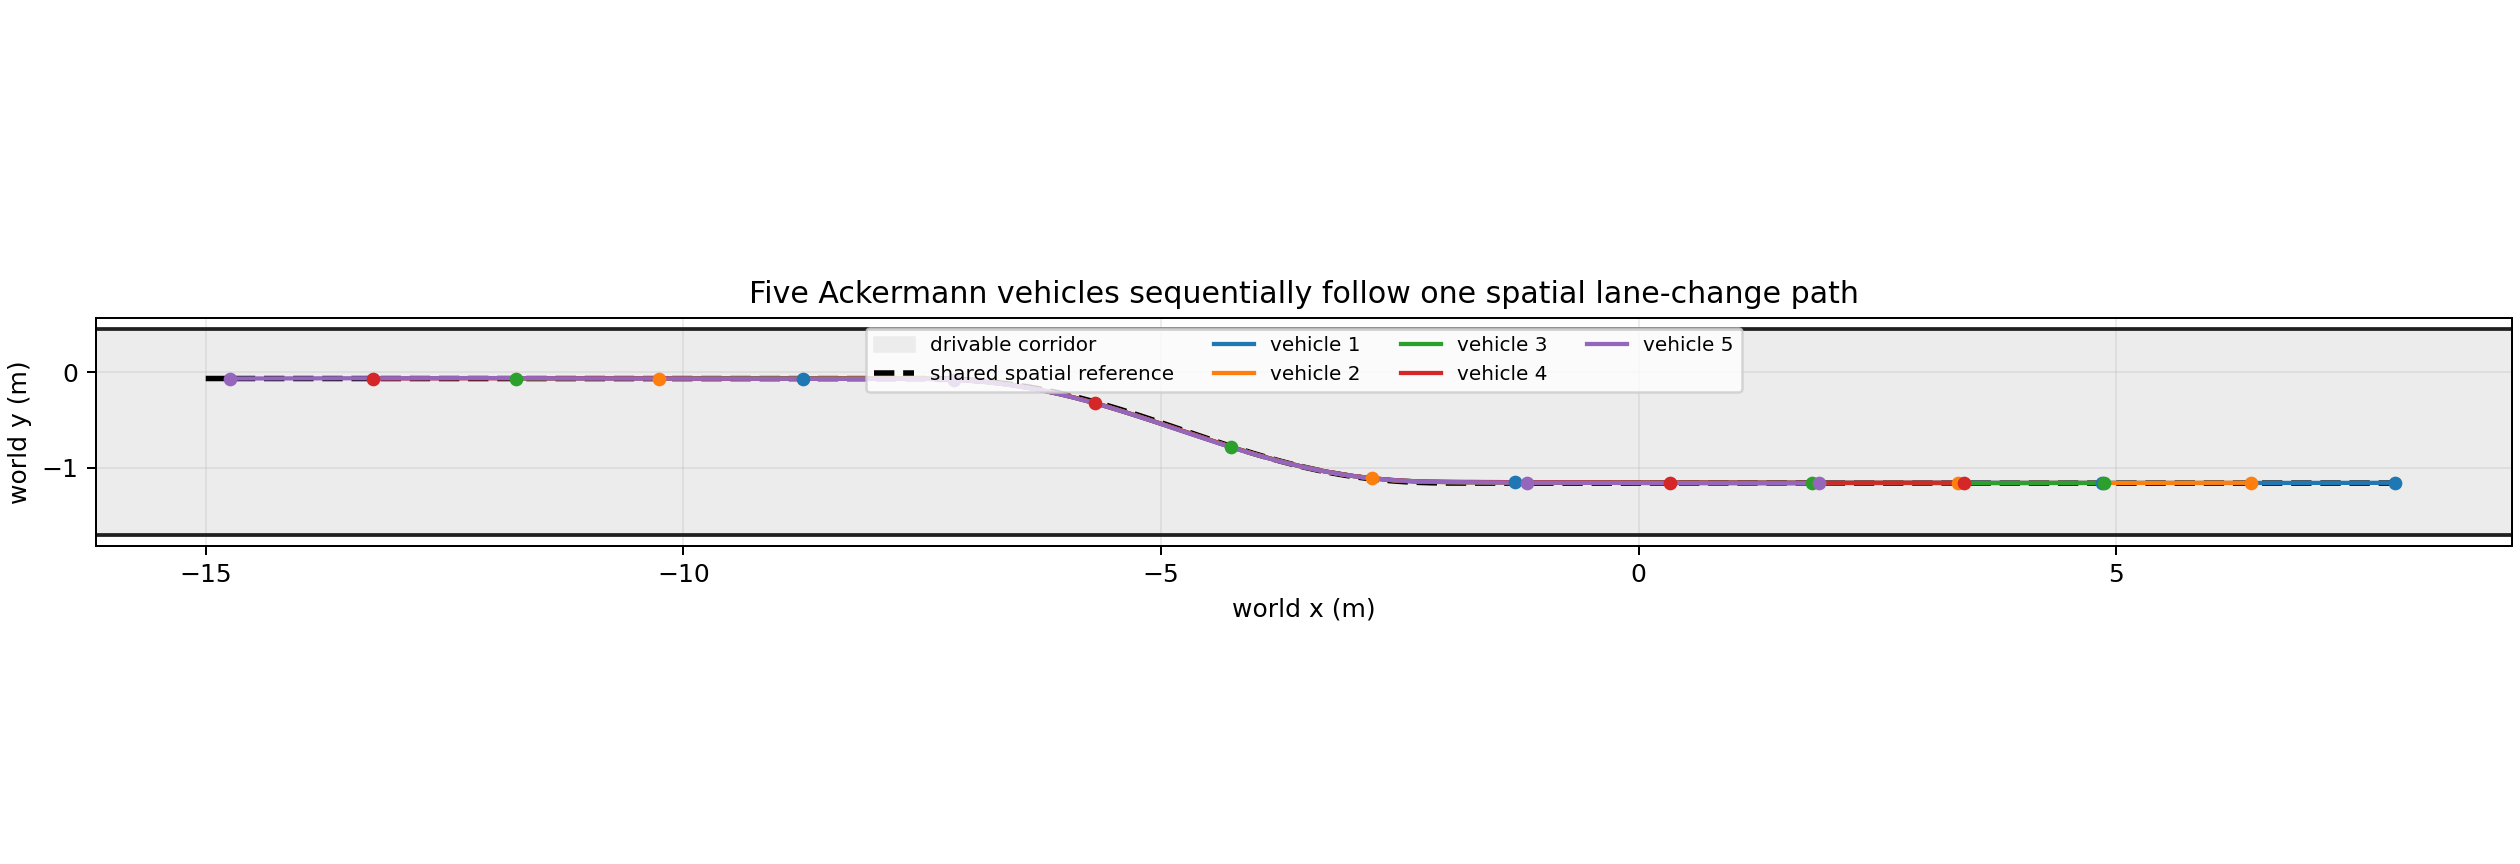
\includegraphics[width=\columnwidth]{figures/five_ackermann_path.png}
\caption{Five Ackermann vehicles sequentially following one shared spatial lane-change path in the real-trajectory evidence.}
\label{fig:commonpath}
\end{figure}

\begin{figure}[t]
\centering
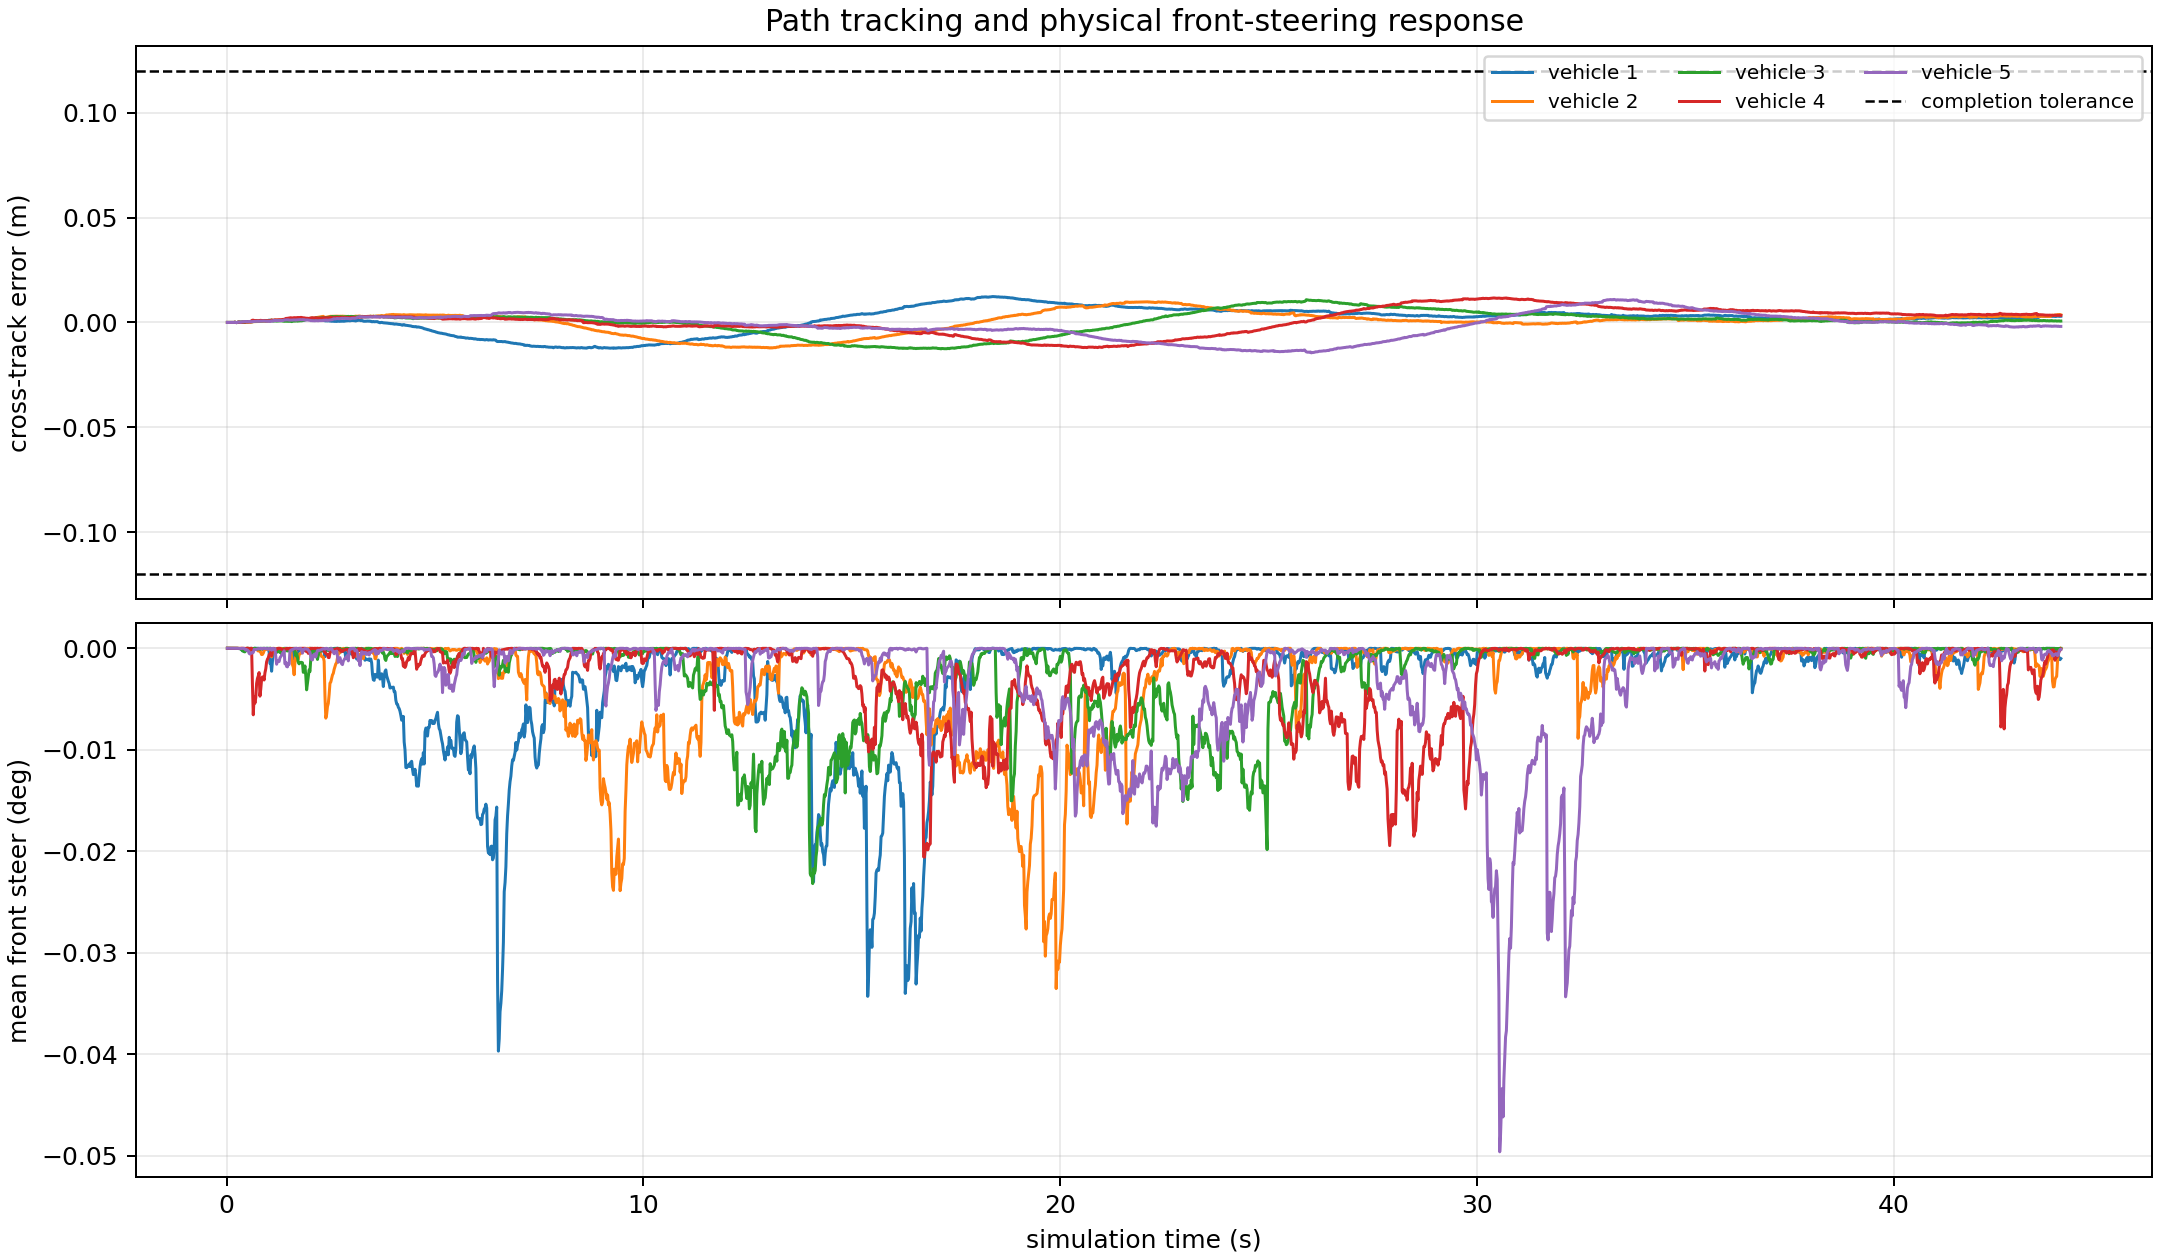
\includegraphics[width=\columnwidth]{figures/ackermann_tracking_steering.png}
\caption{Cross-track error and physical front-steering response for the Ackermann warm-start trajectory.}
\label{fig:ackermann}
\end{figure}

\subsection{Meta-AMS Attack Ladder}
Table~\ref{tab:metaamsladder} reports the completed single-training-chain Meta-AMS ladder from the verified matrix. The policy passes the clean gate and all levels through hard-a. At hard-b, the matrix contains 0.75 whole-platoon completion, with the worst evaluation seed also at 0.75. Collision, road-boundary violation, and road termination are zero in every listed level.

\begin{table*}[t]
\centering
\caption{Verified single-training-chain Meta-AMS ladder.}
\label{tab:metaamsladder}
\scriptsize
\begin{tabular}{lrrrrrrrrr}
\toprule
Level & off & light & easy-0 & easy-a & easy-b & med-a & med-b & hard-a & hard-b\\
\midrule
Completion mean & 1.00 & 1.00 & 1.00 & 1.00 & 1.00 & 1.00 & 1.00 & 1.00 & 0.75\\
Worst seed & 1.00 & 1.00 & 1.00 & 1.00 & 1.00 & 1.00 & 1.00 & 1.00 & 0.75\\
Episode return & 73782 & 71928 & 69744 & 68278 & 66634 & 65198 & 64470 & 61414 & 55884\\
Collision rate & 0 & 0 & 0 & 0 & 0 & 0 & 0 & 0 & 0\\
Road violation & 0 & 0 & 0 & 0 & 0 & 0 & 0 & 0 & 0\\
Road termination & 0 & 0 & 0 & 0 & 0 & 0 & 0 & 0 & 0\\
\bottomrule
\end{tabular}
\end{table*}

\begin{figure}[t]
\centering
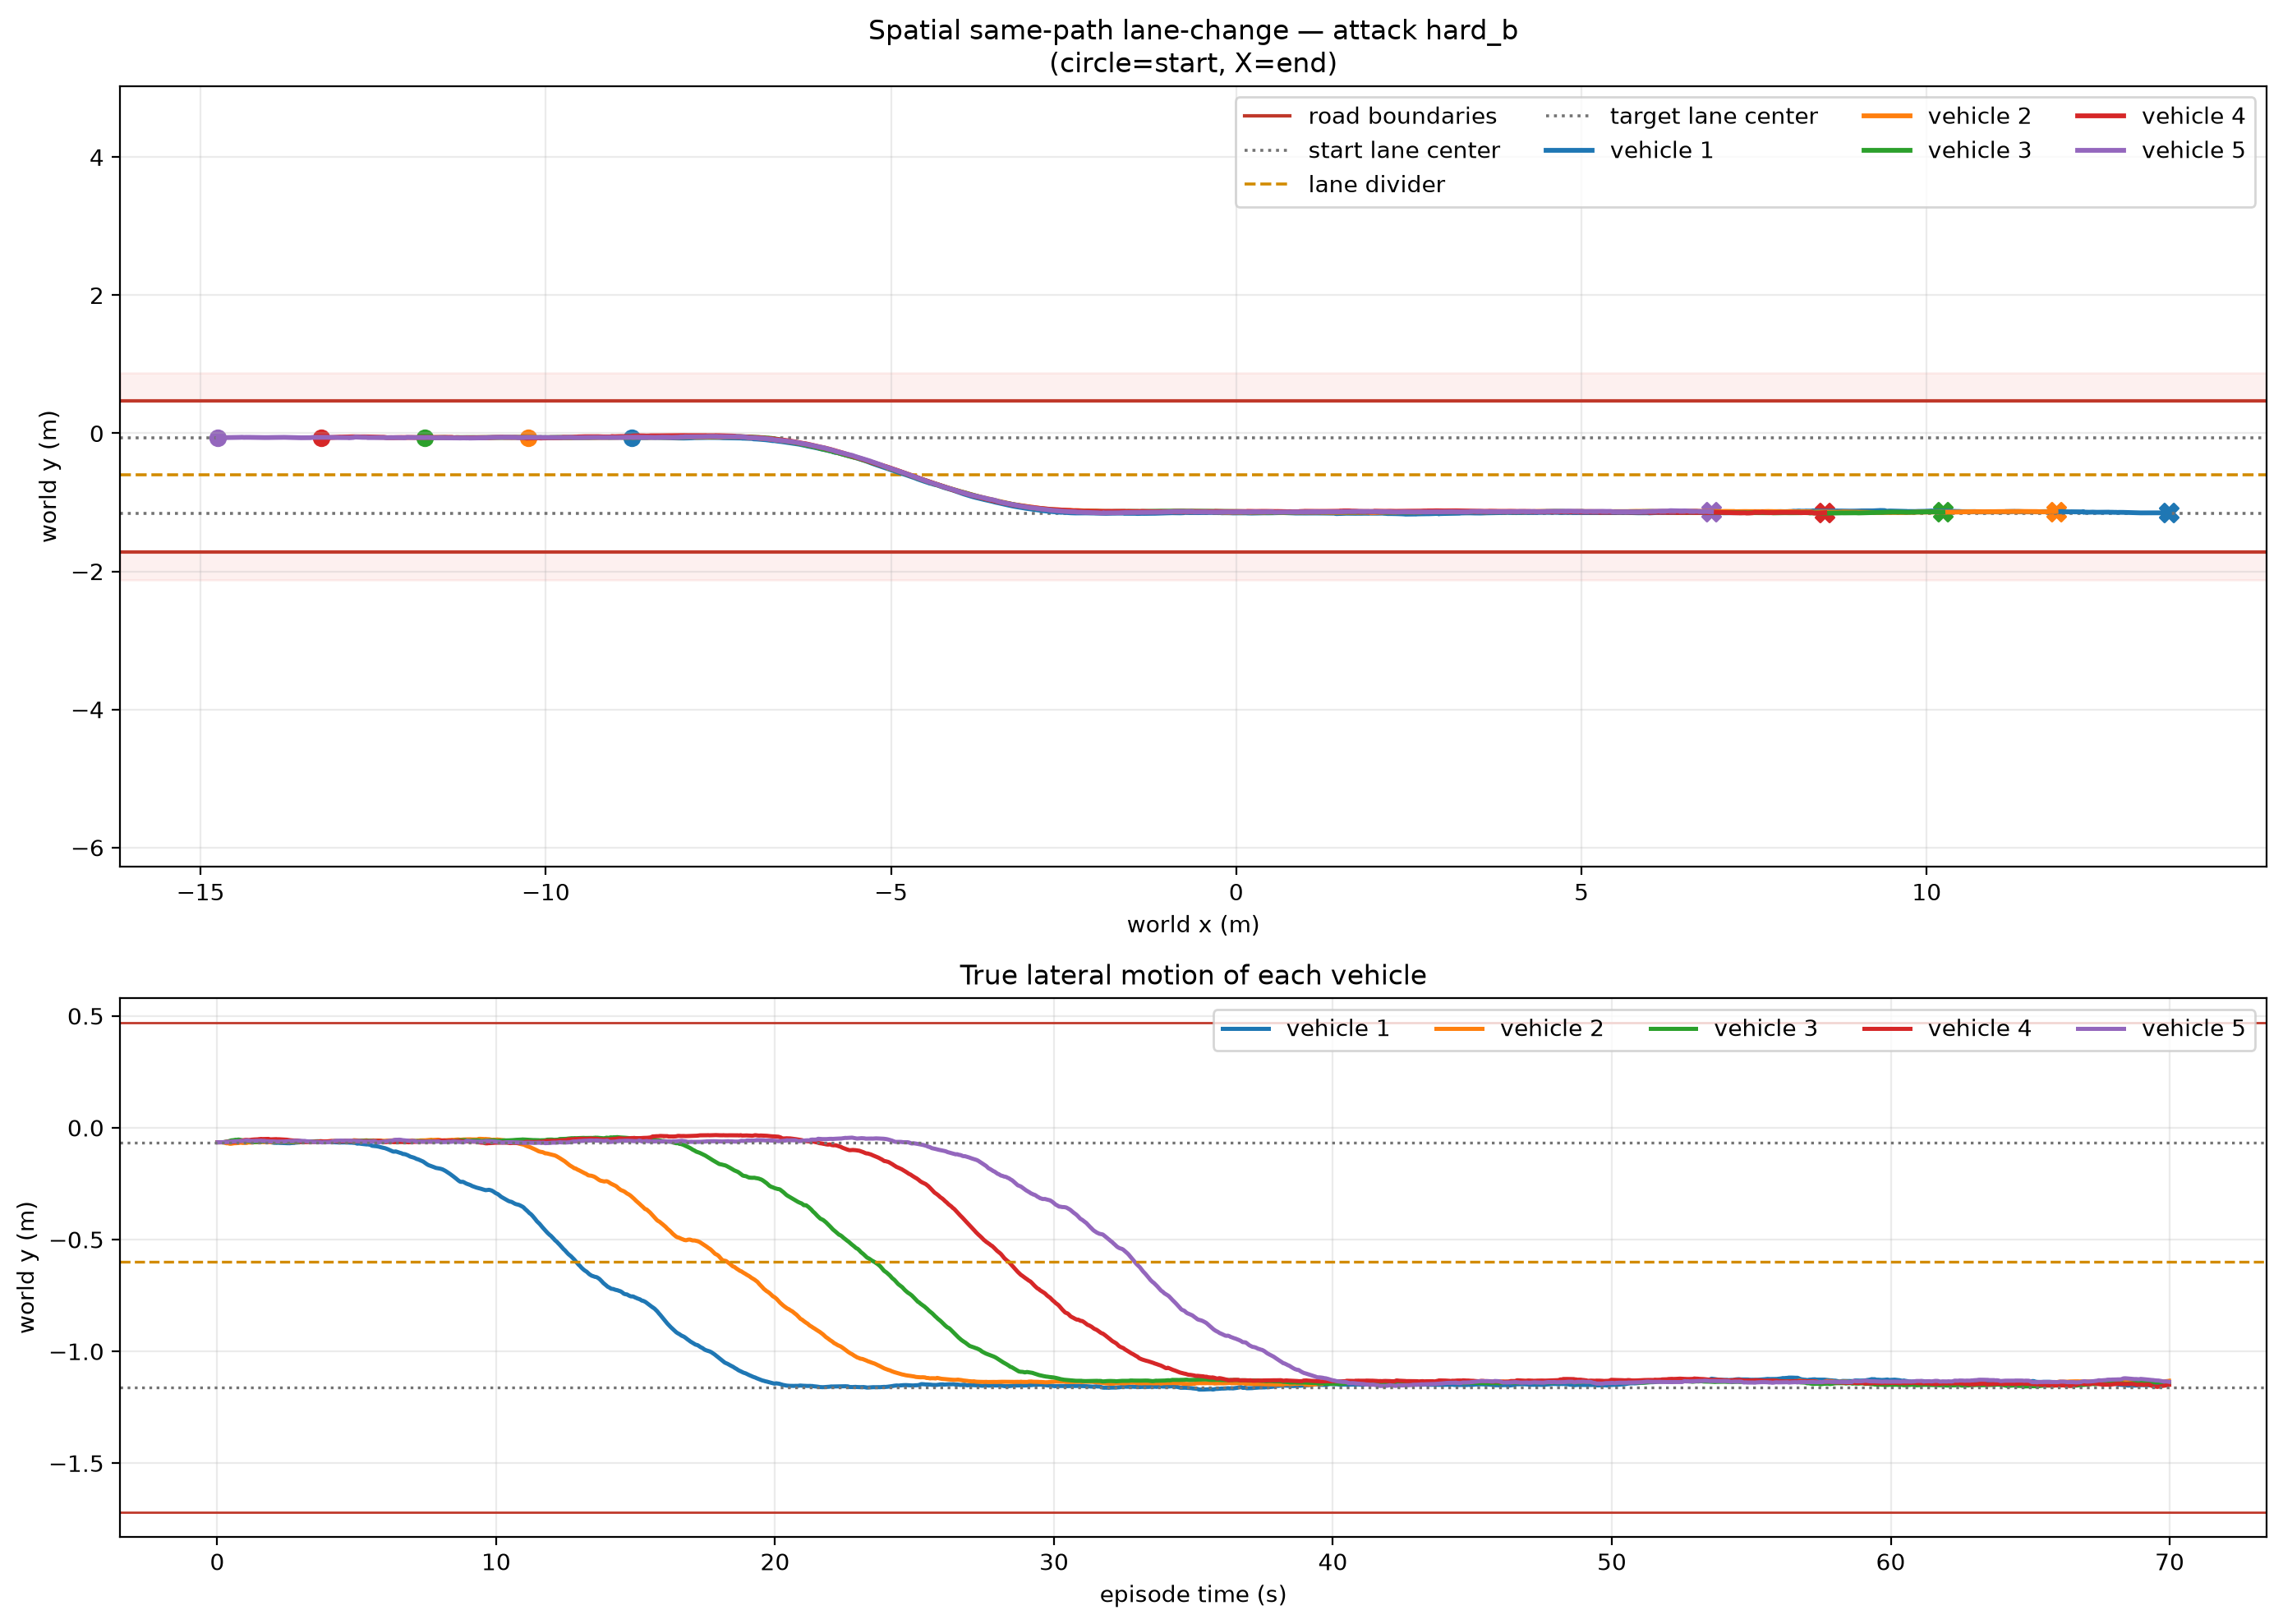
\includegraphics[width=\columnwidth]{figures/meta_ams_hard_b_topdown.png}
\caption{Meta-AMS hard-b top-down trajectory. Circles denote starts and crosses denote final positions; all five vehicles reach the target lane while remaining within the road corridor.}
\label{fig:topdown}
\end{figure}

\begin{figure}[t]
\centering
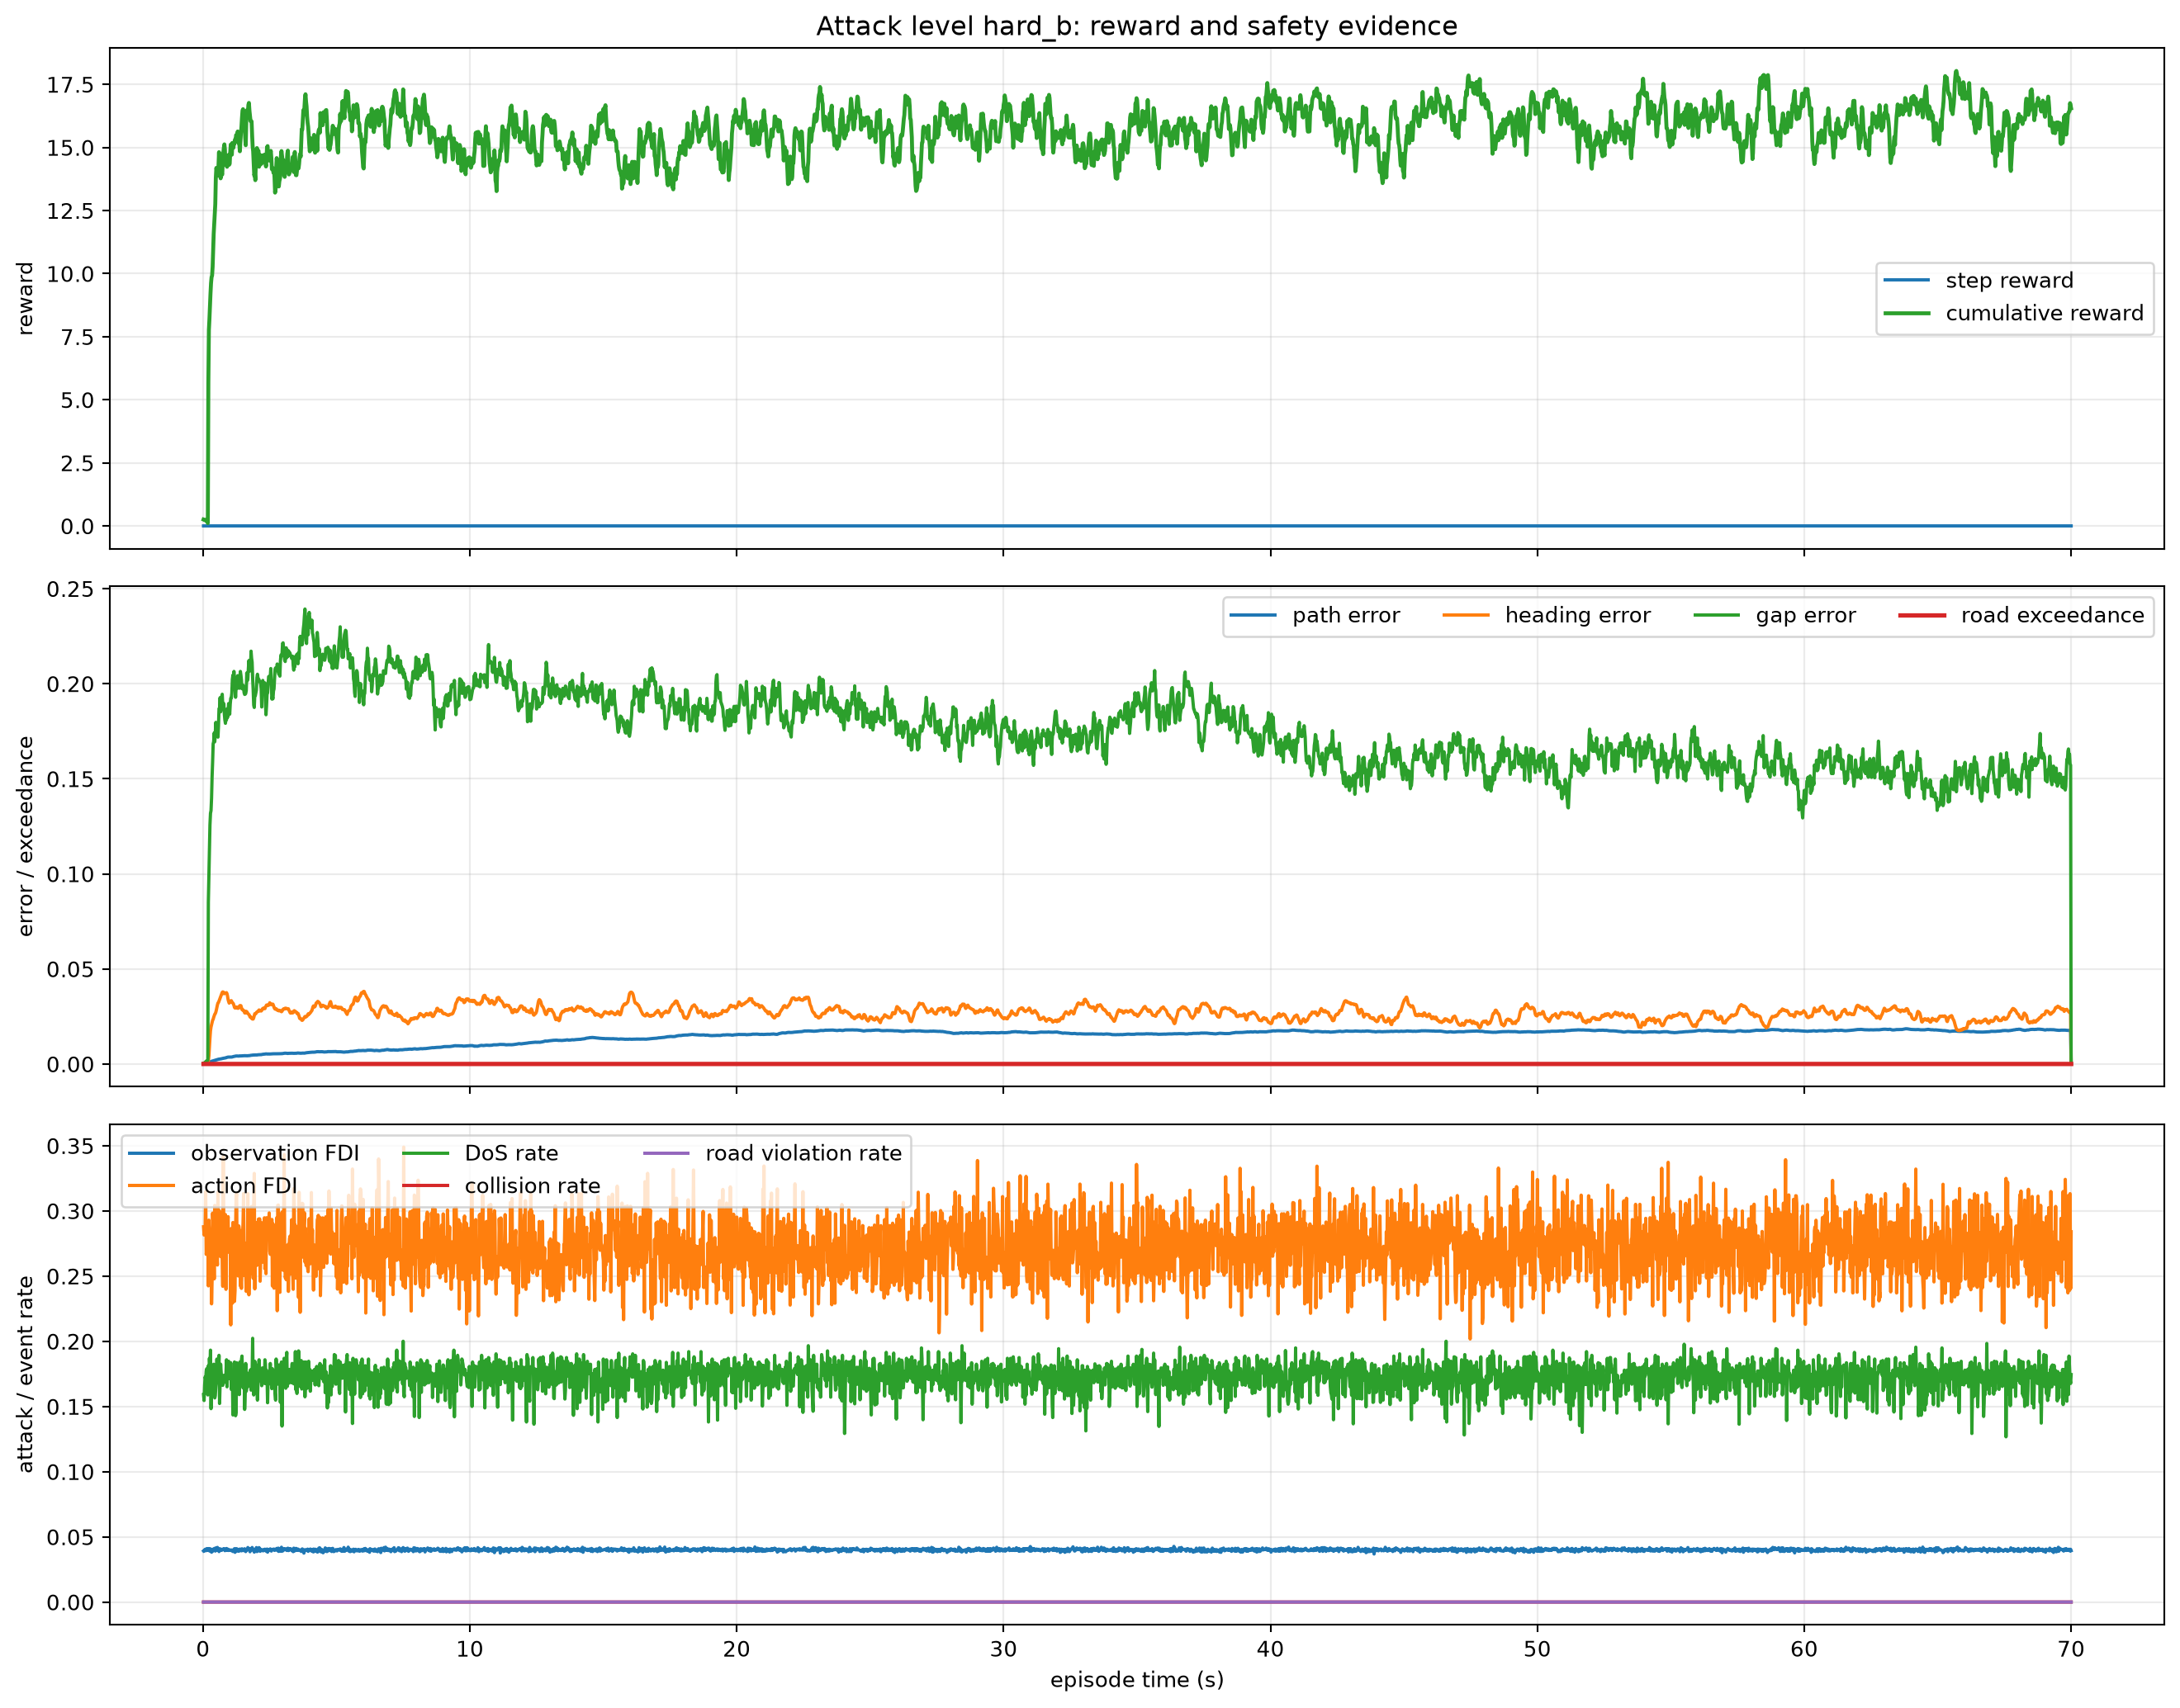
\includegraphics[width=\columnwidth]{figures/meta_ams_hard_b_reward_safety.png}
\caption{Meta-AMS hard-b reward, path/gap/heading errors, and attack/safety signals. The recorded road-exceedance trace remains zero.}
\label{fig:safety}
\end{figure}

\begin{figure}[t]
\centering
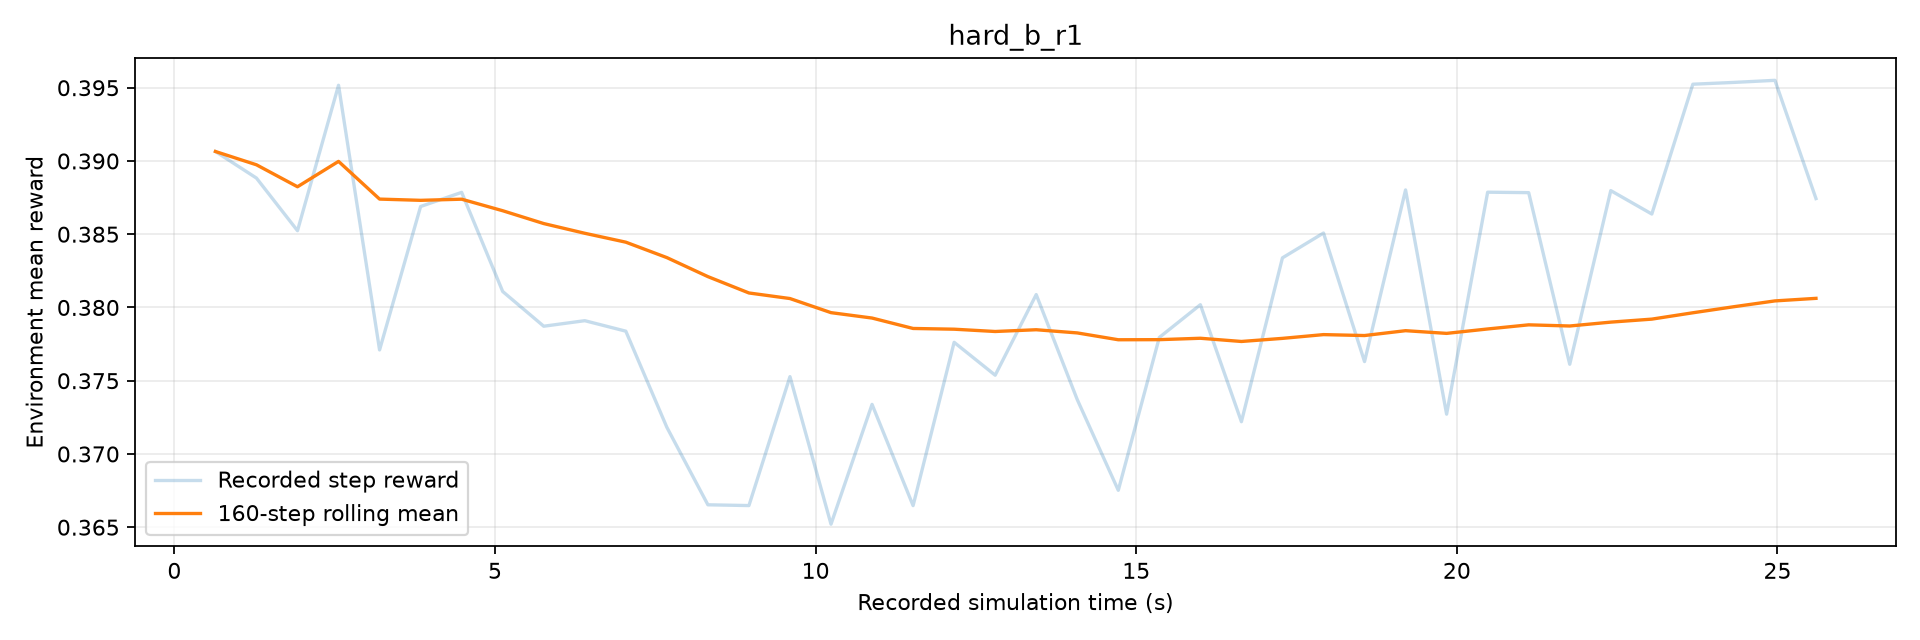
\includegraphics[width=\columnwidth]{figures/meta_ams_training_reward.png}
\caption{Recorded Meta-AMS hard-b stage reward curve and rolling mean.}
\label{fig:reward}
\end{figure}

\subsection{Orthogonal Pilot}
Table~\ref{tab:orthogonal} summarizes the available 2-by-2 pilot. Base shared and Meta-only both reached hard-b with hard-b whole-platoon completion means of 0.5208 and worst-seed rates of 0.50. The full Meta-AMS result reaches 0.75 and passes hard-b. The early AMS-only branch stopped at the light gate. Its hard-b row is an assessment of the last safe BC parent, not a trained AMS-only checkpoint. Moreover, the early branch used a non-shared actor setting; the corrected shared-actor multiseed revalidation is therefore required before a causal standalone-AMS claim.

\begin{table}[t]
\centering
\caption{Current orthogonal pilot at hard-b.}
\label{tab:orthogonal}
\scriptsize
\begin{tabular}{lccc}
\toprule
Method & Completion mean & Worst seed & Training status\\
\midrule
HAPPO base shared & 0.5208 & 0.50 & passed hard-b\\
HAPPO + Meta & 0.5208 & 0.50 & passed hard-b\\
HAPPO + AMS only$^\dagger$ & 0.0417 & 0.00 & stopped at light\\
HAPPO + Meta + AMS & 0.7500 & 0.75 & passed hard-b\\
\bottomrule
\multicolumn{4}{l}{\scriptsize $^\dagger$Diagnostic assessment from the last safe BC parent; not a promoted AMS-only policy.}
\end{tabular}
\end{table}

\begin{figure}[t]
\centering
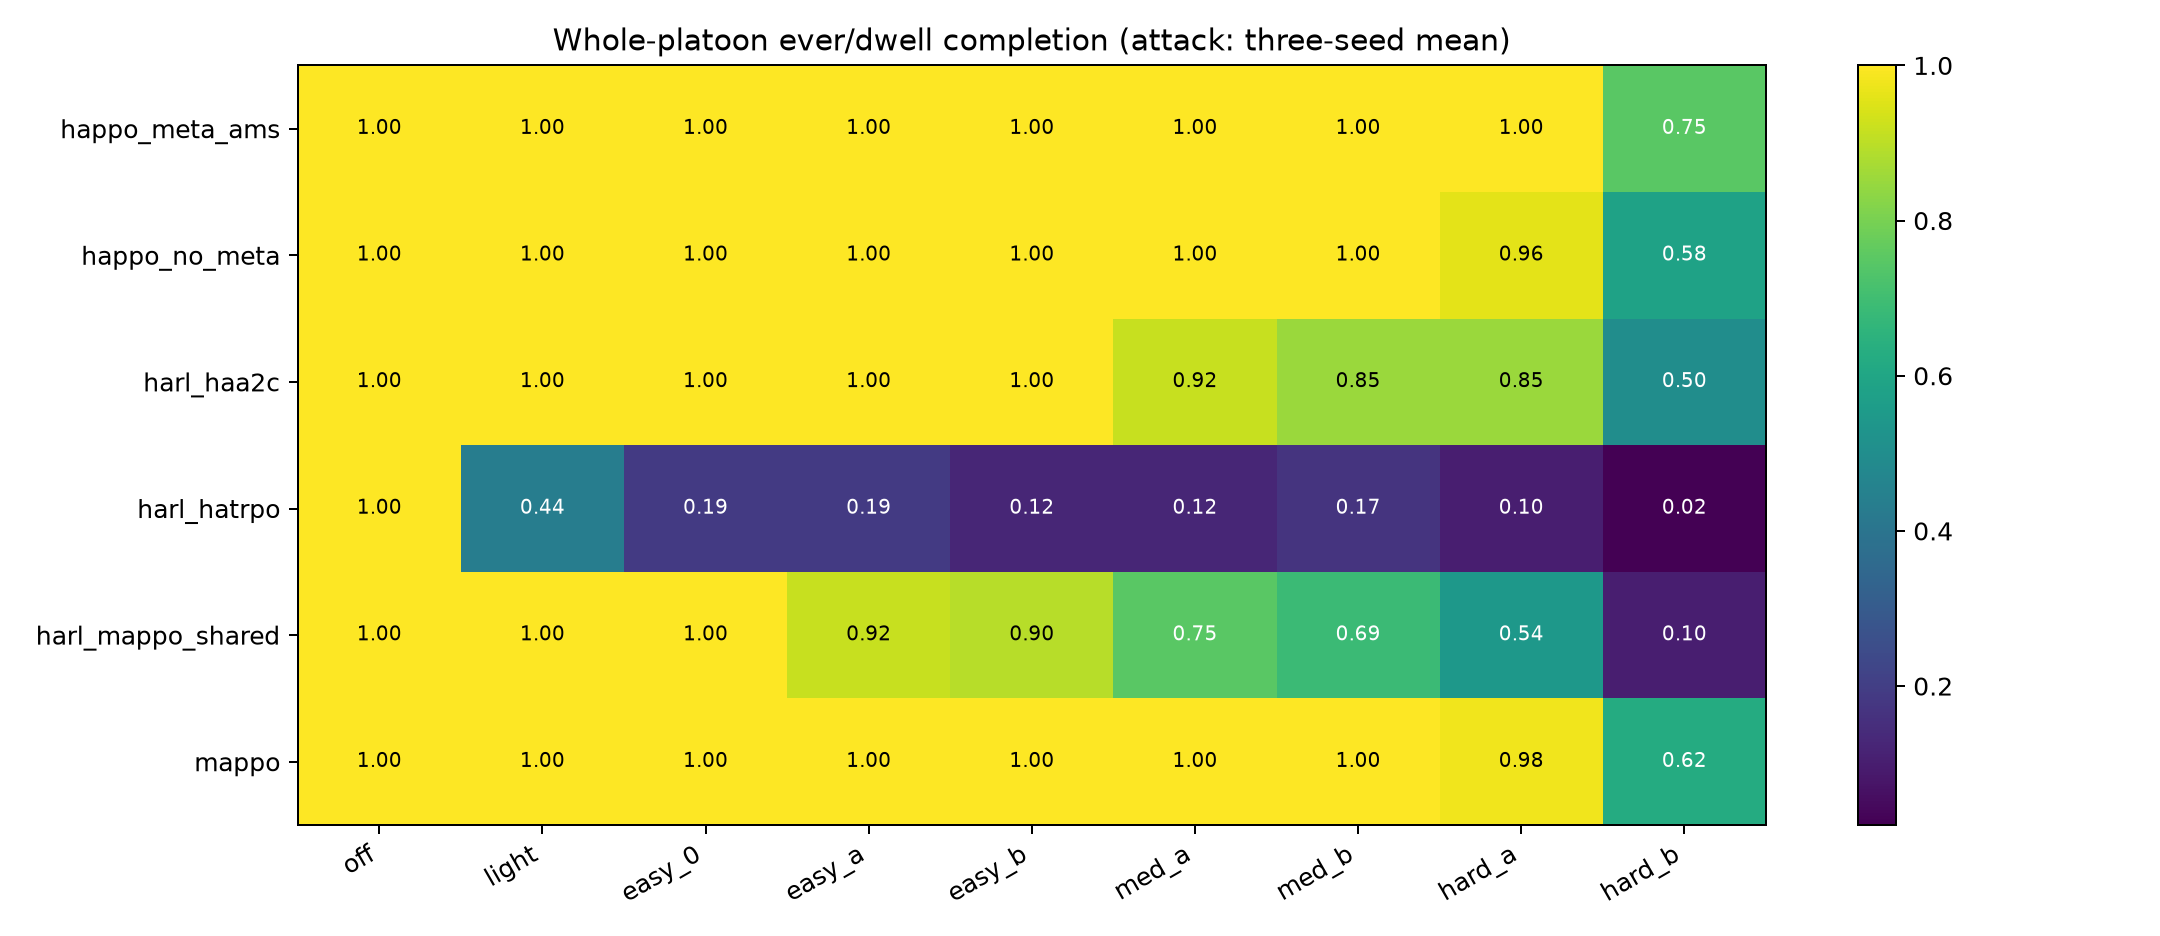
\includegraphics[width=\columnwidth]{figures/six_algorithm_completion_heatmap.png}
\caption{Whole-platoon mean completion over the complete attack ladder for the six-algorithm comparison.}
\label{fig:heatmap}
\end{figure}

\begin{figure}[t]
\centering
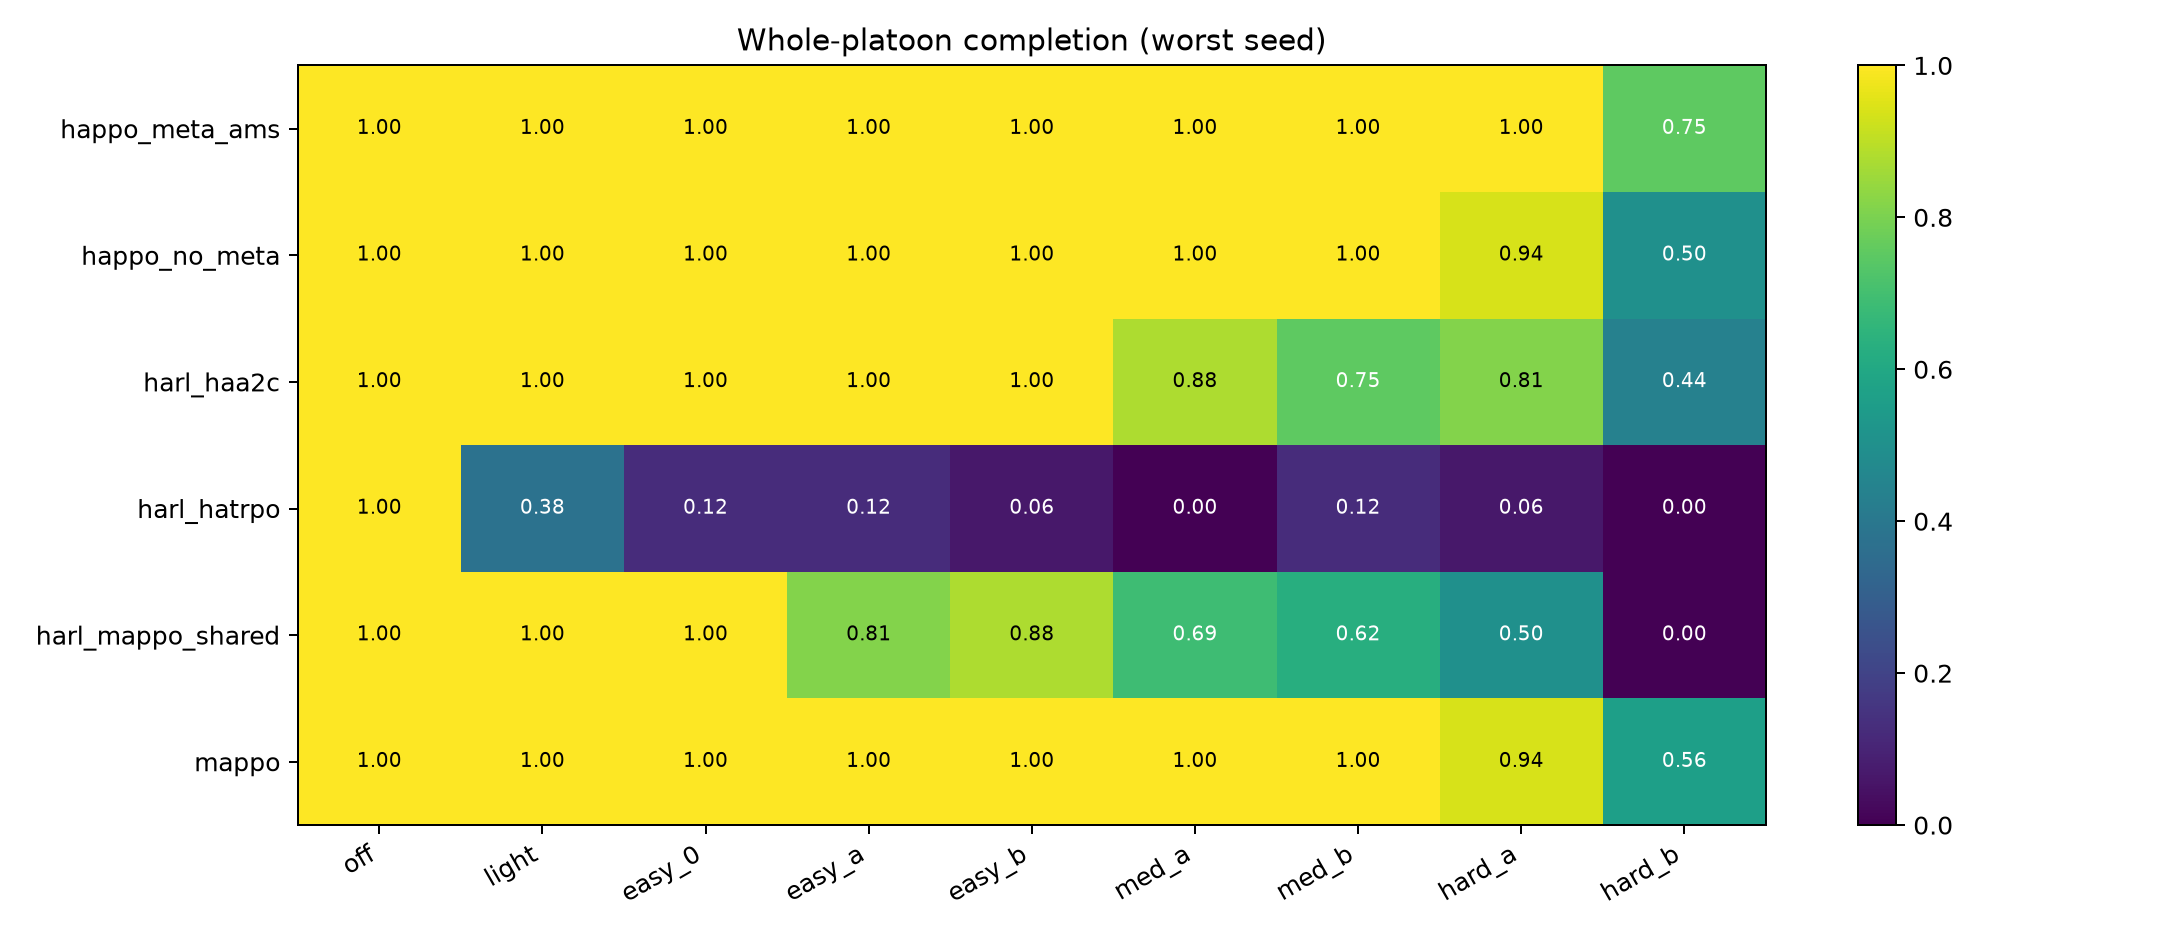
\includegraphics[width=\columnwidth]{figures/six_algorithm_worst_seed_heatmap.png}
\caption{Worst-seed whole-platoon completion over the attack ladder. The worst-seed view exposes the hard-b degradation more clearly than the mean alone.}
\label{fig:worstheatmap}
\end{figure}

\subsection{Comparison with Six Learning Algorithms}
The hard-b comparison in Table~\ref{tab:sixalg} uses the same spatial task, attack ladder, completion gate, and three evaluation seeds. Meta-AMS has the highest current hard-b completion mean and worst-seed rate. The result is evidence for the combined design under the available training chain; it is not yet a multi-seed significance test.

\begin{table}[t]
\centering
\caption{Hard-b comparison from the verified six-algorithm matrix.}
\label{tab:sixalg}
\scriptsize
\begin{tabular}{lccc}
\toprule
Method & Completion mean & Worst seed & Gate\\
\midrule
MAPPO & 0.6250 & 0.5625 & pass\\
HAPPO (no Meta) & 0.5833 & 0.5000 & pass\\
Meta-AMS & 0.7500 & 0.7500 & pass\\
HARL-HAA2C & 0.5000 & 0.4375 & fail\\
HARL-MAPPO shared & 0.1042 & 0.0000 & fail\\
HARL-HATRPO & 0.0208 & 0.0000 & fail\\
\bottomrule
\end{tabular}
\end{table}

\subsection{Interpretation}
The matrix supports three cautious observations. First, the full Meta-AMS policy is the only reported method with a 0.75 hard-b whole-platoon completion rate and a 0.75 worst-seed rate. Second, the safety failures that would be easiest to hide with an average-return metric do not occur in the reported matrix: collision and road termination remain zero. Third, the pilot suggests that the action smoother benefits from a stable Meta-guided task direction. The early AMS-only failure is associated with lower longitudinal gap quality and is not evidence that AMS is intrinsically ineffective, because the branch was architecturally confounded and did not pass the light gate.

\section{Discussion and Limitations}
\subsection{What Meta-AMS Adds to Meta-Gradient Reward Shaping}
The reference MGRS formulation repairs an attack-induced reward mismatch by using trusted physical information in the upper-level update \cite{xia2026security}. Meta-AMS keeps that task-level separation and adds a second, local separation. The teacher chooses a physically meaningful learning direction, whereas AMS evaluates whether a nearby speed--steering action remains valuable and feasible. This division is useful for a nonholonomic platoon: a reward can say that the convoy should reduce gap error, but it does not by itself tell the actor which local steering perturbations preserve curvature and front-wheel consistency.

\subsection{Evidence Boundary}
The completed evidence is based on a single training chain for each reported matrix row and three evaluation seed pairs. Those three attack seeds are evaluation repetitions, not independent training seeds. Independent training-seed replication is running in a separate output root and will be required before reporting confidence intervals, statistical significance, or a definitive interaction effect. The current paper therefore uses the terms pilot, available verified result, and conditional language where appropriate.

\subsection{Theory Boundary}
The local ultimate-boundedness proposition assumes a local dissipative closed loop and bounded admissible attack. It does not prove global stability for arbitrary attack budgets, arbitrary initial spacing, or every learned policy. The simulation gates are designed to test the relevant conditions empirically: shared-path completion, gap maintenance, dwell, collision, and road-boundary constraints. A future revision should estimate the constants in \eqref{eq:uub} from logged trajectories and connect the AMS neighborhood variance to a measurable local robustness margin.

\section{Conclusion}
This paper presented Meta-Guided Action-Manifold Smoothing for secure five-vehicle Ackermann platooning under hybrid DoS--FDI attacks. The method combines a trusted physics-aware Meta Reward Teacher with a feasible, symmetric, twin-critic action neighborhood. The vehicle interface enforces front-wheel steering and rear-wheel drive, while the curriculum begins from real-trajectory imitation and promotes checkpoints only through strict complete-platoon gates. The current verified Meta-AMS chain reaches 0.75 whole-platoon completion at hard-b with zero collision and road-termination rates in the recorded matrix, and the spatial/top-down evidence shows all five vehicles following the same path and completing the lane change. The independent training-seed revalidation remains the next step before making final statistical or causal claims.

\bibliographystyle{IEEEtran}
\bibliography{references/ams}

\end{document}

